\chapter{Project Status}
\label{ch:project-status}

\graphicspath{{mainmatter/project-status/figures/}}

A project timeline is given in \cref{fig:project-status:work-plan}. The project timeline consists of four phases (one preliminary) and seven milestones:

\bigskip
\begin{enumerate}[label=\textbf{Phase \arabic*.},start=0,leftmargin=2.5cm]
  \item \textbf{Early problem investigation.} Early investigation into the problem area, exploring potential aspects for research hypotheses to develop more substantially. The outcome is the first two chapters of this report (Milestone 1) and the early stages of a technical report attached in \cref{appx:tech-report}.
  \item \textbf{Develop initial framework.} Process of developing initial framework by mining developer forums (Stack Overflow) and designing and conduct our surveys. This maps to Experiment I (see \cref{ssec:research-methodology:experiments:2}). The outcome is an initial context-agnostic \gls{cis} \gls{api} documentation quality assessment framework (Milestone 3) and confirmation of candidature complete (Milestone 2). As ethics approval is required, the current draft Ethics Application is attached in \cref{appx:ethics}.
  \item \textbf{Validate initial framework.} Validating that the framework we develop in Phase 1 correctly reflects the needs of developers by trialing it in controlled observational studies. This maps to Experiment II (\cref{ssec:research-methodology:experiments:2}). The outcome is a framework that has been validated against developers (Milestone 4).
  \item \textbf{Finalise framework and thesis.} Implement any additional findings from the validation of Phase 2 into the framework, thereby finalising the framework (Milestone 5). Original contribution is the framework and therefore the thesis can be submitted (Milestone 6) and reviewed before the study is complete (Milestone 7).
\end{enumerate}

\begin{landscape}


\begin{figure}[p!]
  \vspace{-0.5cm}
  \centering
  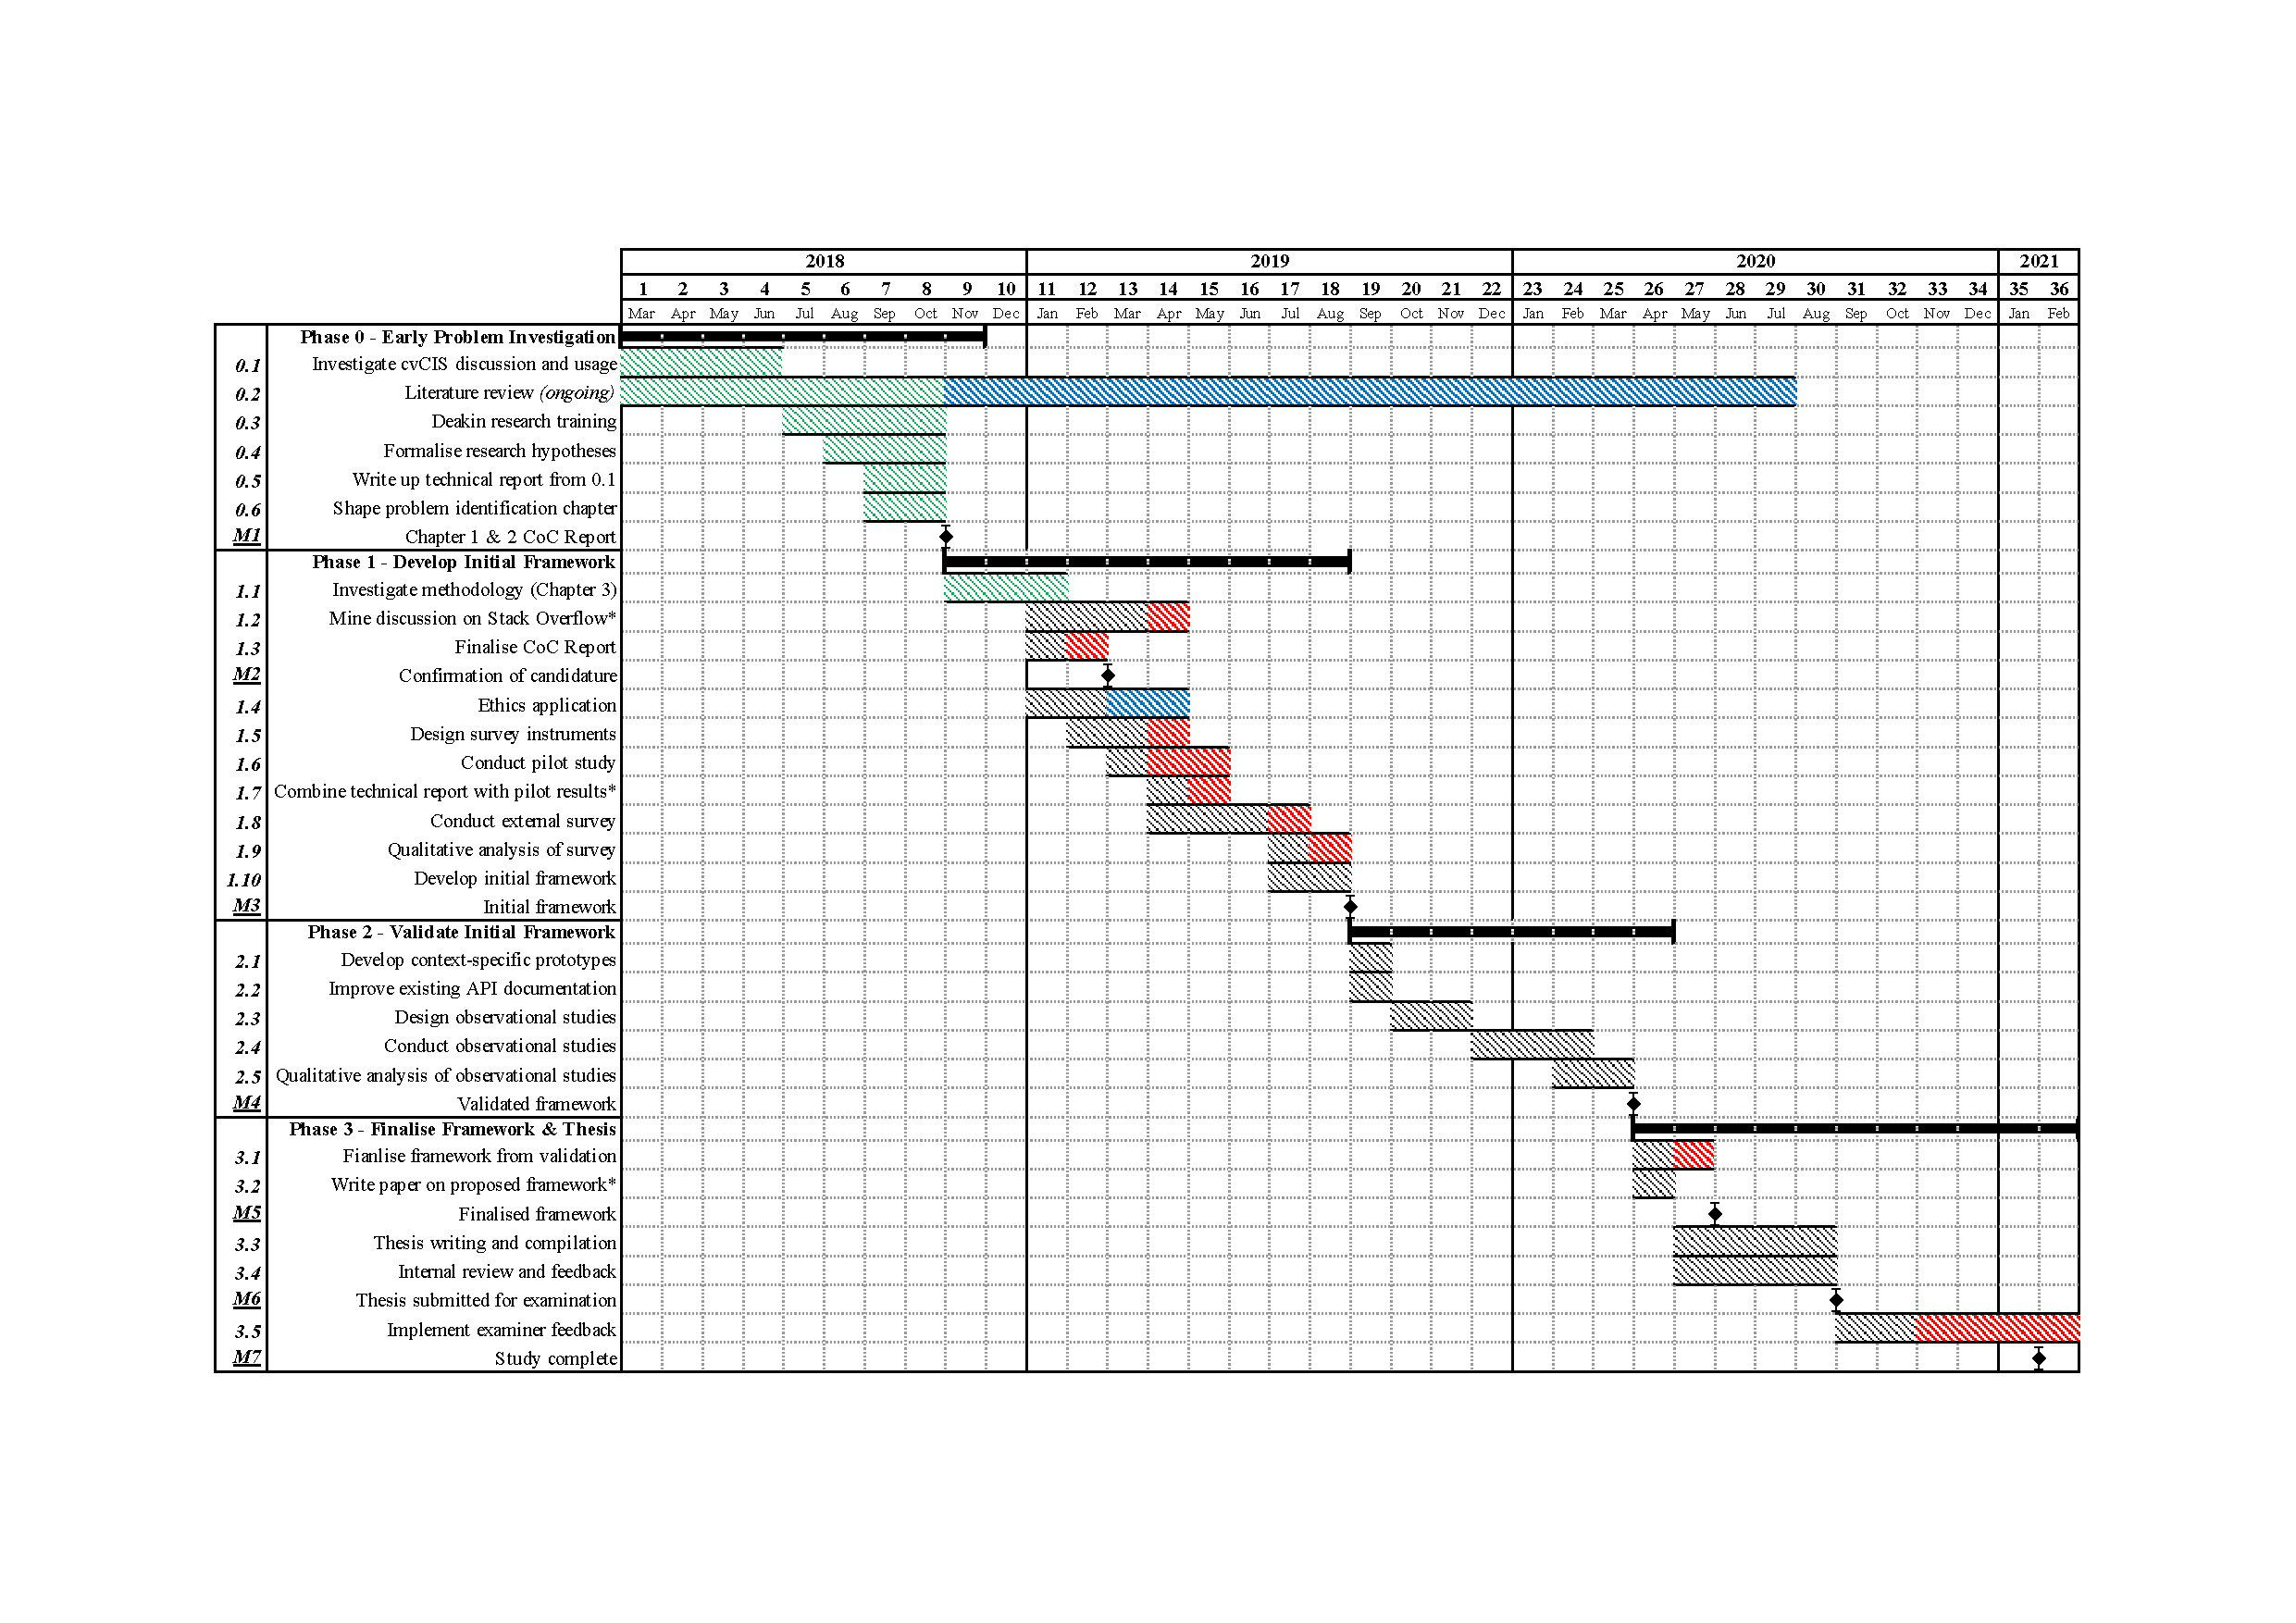
\includegraphics[width=\linewidth]{work-plan}
  \caption[PhD project timeline]{Project timeline. \\ \textit{\textbf{Key:} Green Bar = Completed Task; Grey Bar = Planned Task; Red Bar = Slack Time; Blue Bar = Ongoing Task; Thick Black Line = Phase Duration; Diamond = Milestone; Asterisk = Potential publications.}}
  \label{fig:project-status:work-plan}
\end{figure}
  
\end{landscape}

%\section{Descriptions of Completed Work}
%
%\subsection{Work completed from Phase 0}
%
%\paragraph{Task 0.1 Investigate \gls{cvcis} discussion and usage.} This 
%
%\section{Descriptions of Planned Work}
%
%\subsection{Planned work for Phase 1}
%
%\subsection{Planned work for Phase 2}
%
%\subsection{Planned work for Phase 3}
%\section{Intended Publications}